\documentclass[11pt]{article}

\usepackage{amsmath,amssymb,amsfonts}
\usepackage{booktabs}
\usepackage{graphicx}
\usepackage{hyperref}
\usepackage[margin=1in]{geometry}
\usepackage[numbers,square,sort&compress]{natbib}
\usepackage{algorithm}
\usepackage{algorithmic}
\usepackage{multirow}
\usepackage{xcolor}
\usepackage{tikz}
\usetikzlibrary{positioning,arrows.meta,shapes.geometric,calc}
\usepackage[affil-it]{authblk}

\renewcommand{\arraystretch}{1.3}

\title{Cross-Design Evidence Discordance Diagnoses Phase~III Drug Failure Modes Across Neurodegenerative, Cardiometabolic, and Autoimmune Disease}

\author{Elliot Tower}
\affil{Independent researcher \\ \texttt{elliot@elliottower.ai}}

\date{}

\begin{document}
\maketitle

\begin{abstract}
\textbf{Background:}
The overall failure rate for Alzheimer's disease drug development exceeds 99\%, yet evidence synthesis tools assess consistency within a single study design rather than across designs. We developed a cross-design concordance rule that compares standardized observational and Mendelian randomization (MR) effect sizes to classify mechanism families and diagnose drug failure modes.

\textbf{Methods:}
We assembled 27 mechanism families across three disease domains (neuroepidemiology, cardiometabolic, autoimmune). For each family, observational and MR effect sizes were standardized to Cohen's $d$ using the Chinn formula. A family was classified as discordant when a non-trivial observational association ($d \geq 0.10$) coincided with a null MR signal. We compared four classification rules in an ablation analysis and applied a two-stage design---etiologic evidence only, then adding RCT outcomes---to diagnose failure modes without circularity.

\textbf{Results:}
The rule correctly classified 18 of 22 scored families (7/8 neuroepidemiology, 7/7 cardiometabolic, 4/7 autoimmune). MR-null status alone accounted for all predictive power; MR-only and the cross-design rule produced identical classifications with zero McNemar disagreements. The observational leg was non-trivial ($d \geq 0.10$) for every scored family and added no discriminative information. The two-stage analysis revealed three failure modes: zombie mechanisms (null MR, confounded observational signal), translation gaps (concordant etiologic evidence but null RCT effect), and exposure mismatches (concordant evidence but MR instrument captures a different exposure than the drug). In the autoimmune domain, three approved effector-neutralization drugs (anti-TNF, anti-IL-17, abatacept) showed null MR because their targets are disease consequences rather than causes, defining a mechanistically predictable boundary where MR-based screening is expected to misclassify.

\textbf{Conclusions:}
MR-null status is a strong negative indicator for risk-encoding drug targets. The cross-design framework's contribution is diagnostic rather than predictive: it separates zombie mechanisms, translation gaps, and exposure mismatches that each demand different pipeline responses. For effector-neutralization targets, MR is uninformative and should not be used as a negative screen. This is the first deterministic, parameter-free operationalization of cross-design triangulation validated across three independent disease domains.
\end{abstract}

\paragraph{Keywords:} Mendelian randomization, drug development, evidence synthesis, cross-design concordance, triangulation, Alzheimer's disease, multiple sclerosis, cardiometabolic disease, Phase~III trials, failure-mode diagnosis

\section{Background}

Drug development for Alzheimer's disease and multiple sclerosis consumes billions of dollars annually, with an overall AD drug failure rate exceeding 99\% \cite{cummings2014}. Standard tools for evaluating mechanistic evidence---GRADE for rating certainty, $I^2$ for measuring heterogeneity---operate within a single study design. They assess whether twelve RCTs agree, leaving cross-design consistency untested: whether RCT evidence agrees with genetic evidence, or whether observational signals survive Mendelian randomization.

Several independent findings establish that genetic evidence carries information about drug success. \citet{nelson2015} found that drugs with genetic support for their target are twice as likely to reach approval, a finding refined by \citet{minikel2024} with larger datasets. \citet{gill2021} showed that MR concordance with RCTs predicts drug approval. \citet{ference2019} demonstrated that MR-derived causal estimates for cardiovascular targets match RCT efficacy. Triangulation \cite{lawlor2016} captures the intuition that multiple evidence types with different biases should converge on a true effect, but provides no standard quantitative test and does not distinguish \emph{types} of convergence failure.

We operationalized triangulation with an explicit decision rule and tested it across three disease domains. The results are clarifying: an ablation analysis shows that MR evidence alone accounts for all outcome-predictive power---the observational leg adds zero classifications beyond what MR provides. This negative result has a structural explanation: every mechanism family that reaches Phase~III trials has non-trivial observational support, so the observational variable is constant among scored families and carries no discriminative information.

The contribution is diagnostic rather than predictive. A two-stage analysis---first etiologic evidence only, then adding RCT outcomes---reveals three failure modes that MR alone cannot separate: zombie mechanisms, translation gaps, and exposure mismatches. All produce failed drugs; what differs is \emph{why}.

\paragraph{Contributions.}
\begin{itemize}
\item \textbf{Failure-mode taxonomy (\S\ref{sec:two_modes}).} Three failure modes: zombie mechanisms (null MR, confounded observational signal---the target was never causal), translation-gap mechanisms (concordant etiologic evidence, but intervention insufficient---the target is real, the drug is not), and exposure mismatch (concordant evidence, but the drug does not recapitulate the causal exposure). Each demands a different response and is visible only when observational and interventional evidence are examined alongside MR.
\item \textbf{Ablation (\S\ref{sec:ablation}).} MR-null status alone predicts drug failure as accurately as the full cross-design rule (18/22 correct, zero disagreements). The observational leg does not improve prediction; its value is diagnostic resolution.
\item \textbf{Effector-neutralization boundary (\S\ref{sec:autoimmune}).} In autoimmune disease, approved drugs that neutralize disease effectors (TNF, IL-17) show null MR signals because the effector is elevated as a consequence of disease, not a cause. This defines a mechanistically predictable class where MR-based screening is expected to misclassify, distinguishing it from true zombie mechanisms.
\item \textbf{Amyloid dissection (\S\ref{sec:amyloid}).} Etiologic concordance for amyloid is robust; interventional discordance reveals a translation gap invisible to etiologic or MR evidence alone.
\end{itemize}

\section{Methods}

\subsection{Data}

We assembled 76 neuroepidemiology claims across 24 mechanism families spanning AD and MS. Each claim was coded with its mechanism family, study design (observational, MR, genetic, RCT, diagnostic), effect size estimate, confidence interval, and sample size. Effect sizes on ratio scales were converted to Cohen's $d$ using the \citet{chinn2000} formula:
\begin{equation}
d = \frac{|\ln(\text{OR})| \cdot \sqrt{3}}{\pi}, \qquad
\text{SE}_d = \frac{(\ln\text{CI}_{\text{upper}} - \ln\text{CI}_{\text{lower}})}{2 \times 1.96} \cdot \frac{\sqrt{3}}{\pi}.
\label{eq:chinn}
\end{equation}
Hazard ratios were treated as odds ratios for conversion, an approximation that holds when the outcome is rare; all neuroepidemiology outcomes in this dataset satisfy this condition (AD and MS incidence $< 5\%$ in the study populations). Sources were published systematic reviews, meta-analyses, MR studies, and landmark RCTs. A complete table of all 76 claims with effect sizes, confidence intervals, evidence types, and family assignments is provided in the supplementary materials.

We supplemented the original catalog with etiologic evidence for three families identified through systematic literature search:

\textbf{Anti-CD20-MS.} MR evidence shows that per-SD higher circulating FCRL3 protein is protective against MS (OR~0.83, 95\% CI 0.79--0.89; \cite{lin2023}). Observational B-cell depletion efficacy data from \citet{hu2019}. A CD40 genetic association (OR~1.16; \cite{sokolova2013}) provides corroborating GWAS evidence.

\textbf{HRT-AD.} Observational meta-analysis (protective, OR~0.67, 95\% CI 0.58--0.78; \cite{song2020}) and MR for estradiol (null, OR~1.00, 95\% CI 0.85--1.18; \cite{barth2025}). An ESR1 genetic association (OR~1.14; \cite{cheng2014}) provides corroborating GWAS evidence.

\textbf{Vitamin~D-MS (supplemented).} Observational cohort evidence for low vitamin~D and MS risk (OR~1.40, 95\% CI 1.19--1.64; \cite{munger2006}), added to the existing MR entry.

\subsection{Evidence classification: etiologic versus interventional}

We divided evidence types into two categories. \emph{Etiologic evidence} captures the observational and genetic case for a mechanism: cohort and case-control studies, Mendelian randomization, GWAS, and diagnostic accuracy studies. These ask ``is this mechanism involved in the disease?'' \emph{Interventional evidence} captures the treatment case: randomized controlled trials. These ask ``does intervening on this mechanism help?''

The separation matters because interventional evidence for a mechanism family contains information about the drug outcomes we want to classify. A family's RCT arm is computed from the same trials whose outcomes appear in the holdout. Using it in both places is circular. Etiologic evidence is independent of drug outcomes by construction: neither cohort studies nor MR analyses are causally downstream of whether a drug was approved, so their inclusion in the classification introduces no circularity.

Within etiologic evidence, MR and GWAS studies were pooled into a single ``genetic/causal'' (GEN) evidence type for the concordance rule. This is a pragmatic choice, not an epistemological claim that GWAS susceptibility estimates and MR causal estimates answer the same question---they do not. GWAS estimates disease susceptibility associated with a variant; MR estimates the causal effect of modifying an exposure. The pooling is justified on scale grounds: common variant GWAS effect sizes are inherently small (OR~1.1--1.3 for genome-wide significant hits) even for real causal pathways, and treating them as a separate evidence type would systematically misclassify real GWAS signals as ``null'' against the $d = 0.10$ threshold. The two evidence types in the classification are therefore OBS (observational and diagnostic studies) and GEN (MR and genetic association studies).

\subsection{Cross-design concordance rule}

For each mechanism family, the classification uses two standardized effect sizes: one from observational evidence (OBS) and one from MR/genetic evidence (GEN). When multiple studies exist within a type, we select the most representative published estimate (typically from the largest meta-analysis or most recent MR study). Effect sizes on ratio scales are converted to Cohen's $d$ via Equation~\ref{eq:chinn}. For autoimmune families where case-control standardized mean differences (SMDs) are the natural OBS measure, SMDs enter directly without Chinn conversion.

Each evidence type is classified independently using a two-criterion rule:

\textbf{OBS classification.} Non-trivial if $d_{\text{OBS}} \geq 0.10$; trivial otherwise. The threshold follows Cohen's boundary for negligible effects and is fixed a priori.

\textbf{MR classification.} Causal if (a) the confidence interval excludes the null \emph{and} (b) $d_{\text{MR}} \geq 0.10$; null otherwise. Both criteria must be met---a statistically significant but negligible effect and a large but imprecise effect are both classified as null.

The family-level classification follows from the combination:

\textbf{Qualitative discordance.} OBS non-trivial, MR null. The observational signal does not survive causal testing; the apparent association reflects confounding or reverse causation.

\textbf{Concordance.} OBS non-trivial, MR causal. Both evidence types support the mechanism.

\textbf{Null concordance.} OBS trivial, MR null. No evidence from either type; prediction is ambiguous.

\textbf{Genetic-only signal.} OBS trivial, MR causal. Genetic support without observational confirmation.

This rule operationalizes triangulation \cite{lawlor2016} with an explicit, deterministic decision procedure. Unlike Cochran's $Q$, which assumes all estimates target the same parameter, the concordance rule treats observational and MR estimates as addressing different questions (``is this mechanism associated with disease?'' vs.\ ``is this mechanism causal for disease?'') and classifies their \emph{agreement pattern} rather than testing whether their magnitudes are statistically distinguishable.

\subsection{MR effect-size scaling}

MR effect sizes enter the classification on their native contrast (per-SD, per-unit, or per-genotype). The Chinn $d$ inherits whatever comparison the OR encodes. One family (IL-6R) reports a per-allele OR; this is rescaled to per-SD before Chinn conversion using $\text{OR}_{\text{per-SD}} = \text{OR}_{\text{per-allele}}^{1/\sigma}$ where $\sigma$ is the SD of the exposure per allele. All other MR ORs enter without rescaling. The $d = 0.10$ threshold is applied uniformly across contrasts as a pragmatic choice; we identify threshold-sensitive families in the sensitivity analysis (\S\ref{sec:limitations}).

\subsection{Failure taxonomy}

Three mechanistically defined failure modes follow from the two-stage analysis:

\textbf{Zombie mechanism.} Etiologic evidence is qualitatively discordant---the MR signal is null while the observational association persists. The observational signal reflects confounding or reverse causation; the mechanism is a statistical association, not a causal pathway. Drugs targeting zombies fail because there is nothing causal to intervene on.

\textbf{Translation-gap mechanism.} Etiologic evidence is concordant (the mechanism is genuinely causal), but drugs targeting it fail or produce marginal benefit. The intervention cannot reverse established downstream pathology at the stage of clinical disease. Etiologic evidence alone classifies these as concordant; only RCT evidence reveals the gap.

A third pattern, \textbf{exposure mismatch}, appears when the MR instrument captures a real causal relationship but the drug targets a different exposure window or delivery route (e.g., lifelong genetic vitamin~D status vs.\ adult oral supplementation).

\subsection{Phase~III holdout}

We assembled 38 Phase~III AD and MS drugs with known outcomes (22 failed, 16 approved). For each drug, we mapped its mechanism to a family classification. Drugs whose family lacked classification received no prediction. The rule was mechanical: qualitative discordance (non-trivial OBS, null MR) classifies as failure; concordance (non-trivial OBS, causal MR) classifies as approval.

\subsection{Two-stage analysis design}

\textbf{Stage~1 (de-circularized).} Classify families using only etiologic evidence. All drug outcomes are fully out of sample. This stage can use ``predicts'' language.

\textbf{Stage~2 (retrospective).} Add interventional evidence and reclassify. Drug outcomes are no longer independent of the classification. This stage uses ``is associated with'' language and examines what the additional evidence reveals.

\subsection{Decision rule}

The complete classification procedure is given in Algorithm~\ref{alg:discordance}. The procedure takes published effect sizes as input and returns a family-level classification with no fitted parameters. Each effect size is converted to Cohen's $d$ (ORs via Chinn; SMDs directly). The OBS and MR legs are classified independently against the $d = 0.10$ threshold, and the family classification follows from their combination. The procedure is deterministic, requires no training data, and can be executed by hand with a calculator.

\begin{algorithm}[t]
\caption{Cross-Design Concordance Classification}
\label{alg:discordance}
\begin{algorithmic}[1]
\REQUIRE Mechanism families $\mathcal{F} = \{f_1, \ldots, f_m\}$; for each $f_j$: effect sizes $d_{\text{OBS}}$, $d_{\text{MR}}$, and MR confidence interval $(l, u)$
\medskip
\STATE \textbf{Standardize.} Convert ORs to $d$ via Eq.~\ref{eq:chinn}; SMDs enter directly
\STATE \textbf{Rescale.} If MR OR is per-allele, rescale to per-SD before conversion
\medskip
\FOR{each family $f_j$}
  \STATE \textbf{OBS:} \textsc{Non-trivial} if $d_{\text{OBS}} \geq 0.10$; else \textsc{Trivial}
  \STATE \textbf{MR:} \textsc{Causal} if $1.0 \notin (l, u)$ \textbf{and} $d_{\text{MR}} \geq 0.10$; else \textsc{Null}
  \IF{\textsc{Non-trivial} and \textsc{Null}}
    \STATE $\text{label}(f_j) \leftarrow$ \textsc{Qualitative Discordance} $\rightarrow$ predict \textsc{Failure}
  \ELSIF{\textsc{Non-trivial} and \textsc{Causal}}
    \STATE $\text{label}(f_j) \leftarrow$ \textsc{Concordance} $\rightarrow$ predict \textsc{Success}
  \ELSIF{\textsc{Trivial} and \textsc{Null}}
    \STATE $\text{label}(f_j) \leftarrow$ \textsc{Null Concordance} $\rightarrow$ \textsc{Ambiguous}
  \ELSIF{\textsc{Trivial} and \textsc{Causal}}
    \STATE $\text{label}(f_j) \leftarrow$ \textsc{Genetic-Only} $\rightarrow$ predict \textsc{Success}
  \ENDIF
\ENDFOR
\medskip
\ENSURE For each drug mapped to family $f_j$: predicted outcome $\in \{\textsc{Success}, \textsc{Failure}, \textsc{Ambiguous}\}$
\end{algorithmic}
\end{algorithm}

\subsection{Ablation design}

To test whether the observational leg contributes predictive power beyond MR alone, we compared four classification rules on all scored families (those with known drug outcomes, excluding pending and construct-limited):

\begin{enumerate}
\item \textbf{Always-fail}: predict failure for every family (base-rate baseline).
\item \textbf{MR-only}: predict failure if MR is null, success if MR is causal (ignore OBS).
\item \textbf{OBS-only}: predict success if OBS is non-trivial, failure if OBS is trivial (ignore MR).
\item \textbf{Cross-design}: the full concordance rule (Algorithm~\ref{alg:discordance}).
\end{enumerate}

For each rule we report total accuracy, accuracy split by outcome (correct failures vs.\ correct approvals), and McNemar paired disagreements between the cross-design and MR-only rules---naming the specific families where the rules diverge, if any.

\begin{figure}[t]
\centering
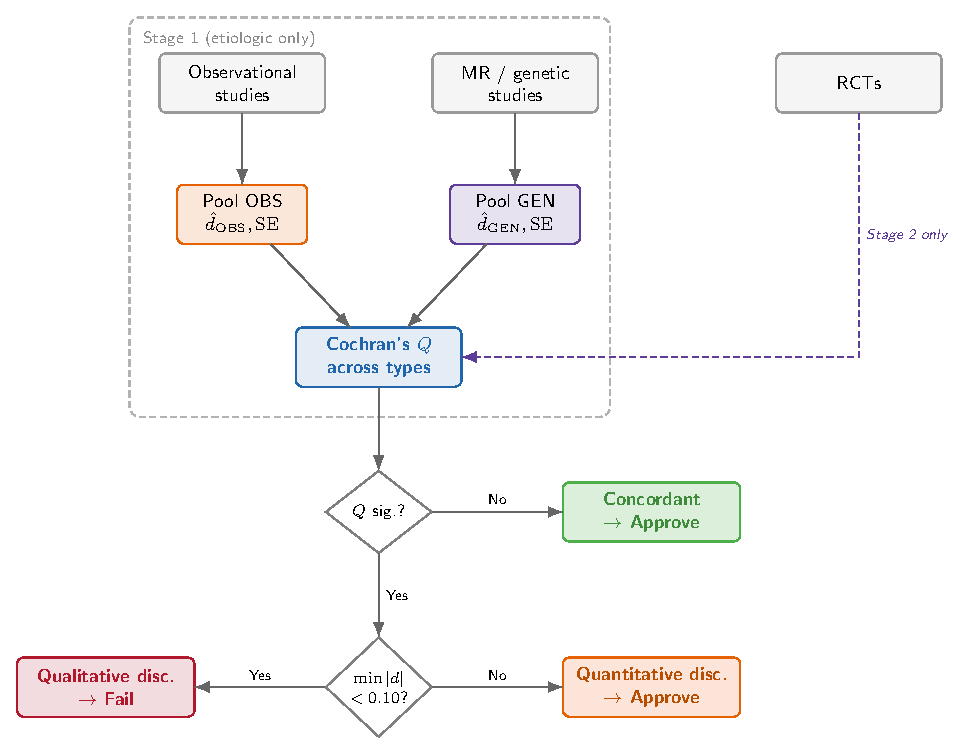
\includegraphics[width=0.85\textwidth]{figures/fig1_flowchart.pdf}
\caption{\textbf{Classification procedure.}
For each mechanism family, observational and MR effect sizes are
standardized to Cohen's $d$ and classified independently against the
$d = 0.10$ threshold. The family-level classification follows from the
OBS$\times$MR combination: qualitative discordance (non-trivial OBS,
null MR) predicts failure; concordance predicts success.
Stage~1 uses etiologic evidence only; Stage~2 adds RCT outcomes to
diagnose failure modes.}
\label{fig:flowchart}
\end{figure}

\section{Results}

\subsection{Family accounting}
\label{sec:accounting}

Table~\ref{tab:accounting} reconciles all denominators used in this paper. We assembled 27 mechanism families across three disease domains. Five are excluded from the scored set: three with pending trial outcomes (BMI-MS, Lp(a), IL-6R), one construct-limited (IL-4R$\alpha$-AD, where the MR instrument and the drug target different ligands), and one ambiguous (uric acid, where MR estimates depend on the method used). The remaining 22 families have unambiguous drug outcomes and enter the ablation and accuracy analyses.

\begin{table}[t]
\centering
\caption{Family accounting across domains. ``Pending'' = no Phase~III readout; ``Constr.'' = construct-limited; ``Ambig.'' = ambiguous MR evidence. The 38-drug holdout (\S\ref{sec:stage1}) is a separate drug-level accounting: of 38 AD/MS drugs, 8 map to 4 etiologically classified neuro families, 14 map to Amyloid-AD (analyzed separately in \S\ref{sec:amyloid}), and 16 map to families without full etiologic classification and receive no prediction.}
\label{tab:accounting}
\small
\begin{tabular}{lccccccc}
\toprule
Domain & Total & Pending & Constr. & Ambig. & Scored & Correct & Accuracy \\
\midrule
Neuroepidemiology & 9 & 1 & 0 & 0 & 8 & 7 & 7/8 \\
Cardiometabolic & 10 & 2 & 0 & 1 & 7 & 7 & 7/7 \\
Autoimmune & 8 & 0 & 1 & 0 & 7 & 4 & 4/7 \\
\midrule
Total & 27 & 3 & 1 & 1 & 22 & 18 & 18/22 \\
\bottomrule
\end{tabular}

\vspace{1mm}
{\footnotesize
Neuro and cardio share the same OBS construct (epidemiological ORs); autoimmune uses case-control SMDs. Domain-specific accuracies are not pooled for inference. The 18/22 total is reported for completeness with the construct-mix disclosure in the abstract.}
\end{table}

\subsection{Stage~1: Etiologic-only classification}
\label{sec:stage1}

Nine neuroepidemiology mechanism families had etiologic evidence from both OBS and MR types; one (BMI~$\to$~MS) is excluded from scoring as prediction pending. Table~\ref{tab:stage1} reports the standardized effect sizes by type and the concordance classification. No interventional data enter this stage.

\begin{table}[t]
\centering
\caption{Stage~1 etiologic-only classification (neuroepidemiology). Five of eight scored families show qualitative discordance: the MR signal is null ($d < 0.10$ or CI spanning null) while the observational association is non-trivial. Three are concordant. BMI~$\to$~MS is excluded as prediction pending. Classification follows Algorithm~\ref{alg:discordance}; no interventional data enter.}
\label{tab:stage1}
\begin{tabular}{lcccccl}
\toprule
Family & MR $d$ & MR CI excl.\ null? & OBS $d$ & OBS class & MR class & Classification \\
\midrule
Metabolic-AD & 0.006 & --- & 0.234 & Non-triv. & Null & Qual.\ disc. \\
ModRisk-AD & 0.053 & --- & 0.209 & Non-triv. & Null & Qual.\ disc. \\
Anti-CD20-MS & 0.103 & Yes & 0.442 & Non-triv. & Causal & Concordance \\
Smoking-MS/AD & 0.016 & --- & 0.209 & Non-triv. & Null & Qual.\ disc. \\
HRT-AD & 0.000 & No & 0.221 & Non-triv. & Null & Qual.\ disc. \\
BMI-AD & 0.016 & Yes$^*$ & 0.393 & Non-triv. & Null & Qual.\ disc. \\
BMI-MS$^\dagger$ & 0.189 & Yes & 0.360 & Non-triv. & Causal & Pending \\
VitD-MS & 0.382 & Yes & 0.186 & Non-triv. & Causal & Concordance \\
EBV-MS & 0.887 & Yes & 0.293 & Non-triv. & Causal & Concordance \\
\bottomrule
\end{tabular}

\vspace{1mm}
{\footnotesize $^*$BMI-AD: CI excludes null (1.01--1.05) but $d = 0.016 < 0.10$, so MR is classified as null under the two-criterion rule.\\
$^\dagger$BMI~$\to$~MS: MR evidence addresses MS susceptibility \cite{mokry2016obesity}; no trial tests a matching clinical endpoint. Excluded from scored count.}
\end{table}

\subsection{Etiologic-only drug classification}

Of 38 holdout AD/MS drugs (22 failed, 16 approved), 8 mapped to 4 families with etiologic classification (Table~\ref{tab:drugs_stage1}). An additional 14 drugs mapped to Amyloid-AD, which is analyzed separately (\S\ref{sec:amyloid}). The remaining 16 drugs mapped to families lacking full OBS$+$GEN evidence and received no prediction.

\begin{table}[t]
\centering
\caption{Etiologic-only drug classification. Accuracy: 7/8 (87.5\%, 95\% Wilson CI: 52.9--97.8\%). Discordant families predicted failure at 100\% (3/3); concordant families predicted approval at 80\% (4/5). Fisher's exact $p = 0.14$; permutation test ($10^5$ shuffles) $p = 0.07$.}
\label{tab:drugs_stage1}
\begin{tabular}{llllc}
\toprule
Family & Classification & Drugs & Outcomes & Correct \\
\midrule
Metabolic-AD & Discordance $\to$ Fail & semaglutide, pioglitazone & Both failed & 2/2 \\
HRT-AD & Discordance $\to$ Fail & CEE/MPA & Failed & 1/1 \\
Anti-CD20-MS & Concordance $\to$ Approve & \parbox[t]{3.2cm}{ocrelizumab ($\times$2),\\ofatumumab,\\ublituximab} & All approved & 4/4 \\
Vitamin~D-MS & Concordance $\to$ Approve & vitamin~D suppl. & Failed & 0/1 \\
\bottomrule
\end{tabular}
\end{table}

The sample is underpowered for frequentist significance at $n = 8$ (Fisher's exact $p = 0.14$; permutation $p = 0.07$), but the directional separation---discordant families producing 100\% drug failure versus 33\% in concordant---is the core finding. Combined with the cardiometabolic replication (\S\ref{sec:cardio}), the rule classifies 14/15 unambiguous neuro+cardio outcomes correctly across two independent disease domains (combined permutation $p = 0.001$). A third domain (autoimmune) provides 4/7, with three misses that define the effector-neutralization boundary (\S\ref{sec:autoimmune}).

The single miss exemplifies \emph{exposure mismatch}: the MR instrument measures the causal effect of one exposure (lifelong genetically determined vitamin~D status), while the drug delivers a different one (adult oral supplementation). These are different interventions on the same pathway, and concordance between MR and observational evidence does not guarantee that the drug recapitulates the exposure the instrument captures. For vitamin~D-MS, MR supports a causal role for lifelong status (OR~2.0, $d = 0.38$) and observational evidence agrees (OR~1.40, $d = 0.19$), producing concordance and predicting approval. The trial failed because adult supplementation does not recapitulate lifelong exposure. This failure mode is predictable a priori whenever the MR instrument's exposure window diverges from the drug's mechanism of action---it is a structural property of the instrument-intervention mapping, not a quirk of one family.

\paragraph{Prediction pending: BMI and MS.}
BMI~$\to$~MS occupies a distinct category: the etiologic evidence supports causation, but no randomized trial has tested the corresponding clinical endpoint. Two-sample MR estimates a causal effect on MS \emph{susceptibility} (inverse-variance-weighted OR 1.41 per SD BMI, 95\% CI 1.20--1.66; \cite{mokry2016obesity}), though the pleiotropy-robust weighted-median estimate attenuates toward null (OR 1.26, 0.98--1.62). The interventional literature does not close this gap: behavioral weight-loss trials achieve substantial weight reduction (8.6\% vs.\ 0.7\% in MoDEMS) but measure mobility, fatigue, and quality of life rather than relapse rate, disability accrual, or incidence \cite{bruce2023modems}, and calorie-restriction RCTs are powered on biomarkers such as serum leptin \cite{ghezzi2025icr}. Because the etiologic claim (onset) and the trial endpoints (symptoms, surrogates) address different constructs, BMI~$\to$~MS is excluded from the scored concordance count.

By contrast, BMI~$\to$~AD enters as a scored family: MR evidence shows a near-null causal effect (OR 1.03, 95\% CI 1.01--1.05; $d = 0.016$) against a strong observational association (midlife obese vs.\ normal BMI: RR 2.04, 95\% CI 1.59--2.62, $d = 0.39$; \cite{anstey2011}), producing qualitative discordance and correctly predicting that weight-loss interventions would not prevent AD.

\subsection{Cases etiologic evidence diagnoses}

\paragraph{Metabolic-AD (zombie mechanism).} T2D associates with AD in observational cohorts (RR~1.53, $d = 0.24$). MR finds no causal effect (OR~1.01, $d = 0.006$). The 40-fold gap diagnoses confounding: shared risk factors (obesity, inflammation, vascular disease) explain the association without a causal metabolic pathway. Semaglutide's null results in EVOKE/EVOKE+ confirmed this classification. Pioglitazone also failed.

\paragraph{HRT-AD (zombie mechanism).} A meta-analysis of 16 observational studies shows HRT is protective against AD (OR~0.67, $d = 0.22$; \cite{song2020}). MR for estradiol finds no causal effect (OR~1.00; \cite{barth2025}). The WHIMS trial found HRT \emph{increased} dementia risk (HR~1.76; \cite{shumaker2003}). The observational protective signal reflects healthy-user bias. The concordance rule correctly identifies this discordance before any RCT data enters the classification.

\paragraph{Anti-CD20-MS (concordance, real mechanism).} MR evidence shows that per-SD higher circulating FCRL3 protein is protective against MS (OR~0.83, $d = 0.103$; \cite{lin2023}). Observational B-cell depletion efficacy data shows a large effect ($d = 0.44$; \cite{hu2019}). Both types exceed the 0.10 threshold---the mechanism is supported across evidence types. GWAS evidence (CD40, OR~1.16; \cite{sokolova2013}) corroborates B-cell involvement. All four Anti-CD20 drugs in the holdout were approved. A caveat on instrument-target alignment: the MR instrument captures circulating FCRL3-mediated B-cell biology, while ocrelizumab depletes CD20$^+$ B cells via antibody-dependent cellular cytotoxicity---a related but distinct mechanism. This family's MR $d = 0.103$ clears the threshold by 0.003; at $d = 0.099$ the classification would flip to discordance and predict failure for all four approved drugs. This threshold sensitivity is discussed in the Limitations (\S\ref{sec:limitations}).

\subsection{The case etiologic evidence cannot diagnose: amyloid}
\label{sec:amyloid}

Amyloid-AD has only observational etiologic evidence in the catalog (amyloid PET positivity strongly predicts AD conversion: HR~3.74 and 10.2). Genetic evidence for amyloid's role in AD is strong: APOE4 heterozygous OR~3.46, homozygous OR~15.65, and APP/PSEN mutations cause autosomal dominant AD. If classified on etiologic evidence, Amyloid-AD would be concordant. The classification would predict approval. And 12 of 14 amyloid-targeting drugs failed Phase~III.

This is a translation gap. The etiologic case is correct: amyloid is involved in AD pathogenesis. The therapeutic failure suggests that clearing amyloid at the stage of clinical disease does not reverse the downstream pathology---plausibly because tau propagation, synaptic loss, and neuroinflammation have become self-sustaining, though this mechanistic explanation remains a hypothesis. What the data show directly is that RCT $d = 0.04$ against etiologic $d > 0.80$: the intervention achieves far less than the etiologic evidence predicts. Etiologic concordance does not guarantee interventional success.

\subsection{Stage~2: Retrospective analysis including RCT evidence}
\label{sec:stage2}

Adding RCT evidence to the etiologic classification reveals which concordant families nonetheless produce drug failures---the translation-gap signature. Amyloid-AD exemplifies this: concordant etiologic evidence, but RCT $d = 0.04$ against etiologic $d > 0.80$ (Table~\ref{tab:stage2}).

\begin{table}[t]
\centering
\caption{Stage~2 retrospective analysis including RCT evidence. Adding RCT $d$ reveals translation-gap mechanisms: families with concordant etiologic evidence (OBS and GEN both non-trivial) but near-zero RCT effect. Amyloid-AD is the clearest example (RCT $d = 0.04$ against OBS $d = 0.86$). This analysis is retrospective---the RCT evidence derives from the same trials whose outcomes appear in the drug set.}
\label{tab:stage2}
\begin{tabular}{lcccl}
\toprule
Family & OBS $d$ & GEN $d$ & RCT $d$ & Failure mode \\
\midrule
Metabolic-AD & 0.24 & 0.006 & 0.00 & Zombie \\
ModRisk-AD & 0.20 & 0.053 & --- & Zombie \\
HRT-AD & 0.22 & 0.000 & 0.34$^*$ & Zombie \\
Anti-CD20-MS & 0.44 & 0.103 & 0.20 & --- (success) \\
Smoking-MS/AD & 0.21 & 0.016 & --- & Zombie \\
BMI-AD & 0.39 & 0.016 & --- & Zombie \\
VitD-MS & 0.19 & 0.382 & 0.19 & Exposure mismatch \\
EBV-MS & 0.29 & 0.887 & --- & --- (success) \\
Amyloid-AD & 0.86 & --- & 0.04 & Translation gap \\
\bottomrule
\end{tabular}

\vspace{1mm}
{\footnotesize $^*$HRT-AD RCT $d = 0.34$ is in the \emph{harmful} direction (WHIMS: HR 1.76 for dementia). The sign reversal---observational protection, RCT harm---is the strongest zombie signature in the dataset.}
\end{table}

The key revelation from adding RCT evidence: Amyloid-AD's near-zero RCT effect ($d = 0.04$) against its strong observational signal ($d = 0.86$) is the signature of a translation-gap mechanism. Etiologic concordance predicted success; 12 of 14 drugs failed. This gap between etiologic concordance and interventional failure is invisible without RCT evidence.

\subsection{Amyloid subanalysis}

Amyloid-AD contained 14 holdout drugs: 12 failed, 2 approved (lecanemab, donanemab). Within the family, production-pathway inhibitors (BACE inhibitors, gamma-secretase inhibitors/modulators) failed at 100\% (8/8). Amyloid immunotherapy failed at 67\% (4/6). Production-pathway inhibition---blocking the enzymes that generate amyloid---consistently produced null or harmful results (semagacestat worsened cognition). The immunotherapy approach achieves amyloid clearance with statistically significant but clinically marginal benefit (27--35\% slowing on CDR-SB).

\subsection{Failure-mode taxonomy}
\label{sec:two_modes}

The two-stage analysis reveals three structurally distinct ways mechanisms fail:

\textbf{Zombie mechanisms} (caught by the concordance rule): the MR signal is null. The observational association reflects confounding or reverse causation. Etiologic evidence alone diagnoses the failure, and drugs targeting the mechanism will fail because there is nothing causal to intervene on. Examples: Metabolic-AD (semaglutide), HRT-AD (WHIMS).

\textbf{Translation-gap mechanisms} (visible only with RCT evidence): the etiologic case is concordant---the mechanism is genuinely involved in the disease. Drugs targeting it still fail because the intervention cannot reverse downstream pathology. The concordance rule classifies these as concordant (predicting success); only interventional evidence reveals the gap. Example: Amyloid-AD.

A third pattern, \textbf{exposure mismatch}, appears when the MR instrument captures a biologically real causal relationship but the drug intervention targets a different exposure window or delivery mechanism. Vitamin~D-MS exemplifies this: lifelong genetic vitamin~D status is causal for MS risk, but adult oral supplementation does not recapitulate the lifelong exposure.

The practical implication: a null MR signal for a drug target is a strong negative signal---the mechanism is likely a zombie. A positive MR signal is necessary but insufficient---the mechanism is real, but translation is not guaranteed, and the match between the MR instrument and the drug's mechanism of action must be evaluated separately.

\begin{figure}[t]
\centering
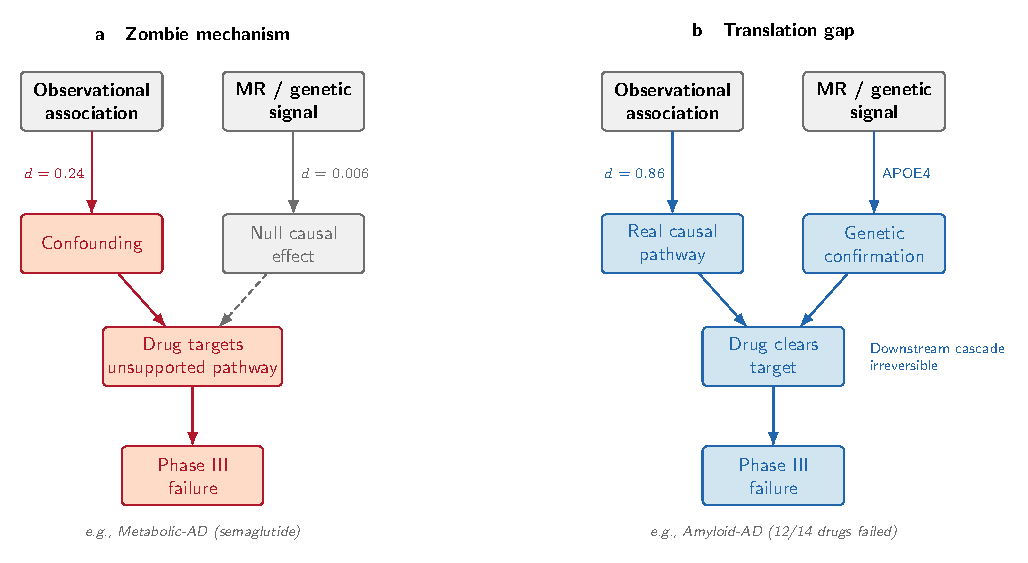
\includegraphics[width=\textwidth]{figures/fig2_failure_modes.pdf}
\caption{\textbf{Three failure modes.}
\textbf{a},~Zombie mechanisms: the observational association ($d = 0.24$
for Metabolic-AD) reflects confounding; the MR/genetic signal is null
($d = 0.006$). Drugs target a phantom pathway and fail Phase~III.
\textbf{b},~Translation-gap mechanisms: both observational and genetic
evidence confirm the pathway is real (Amyloid-AD, APOE4 OR~$= 3.46$),
but the downstream neurodegenerative cascade is irreversible by the time
of intervention. Twelve of fourteen amyloid-targeting drugs failed.
\textbf{c},~Exposure mismatch: etiologic evidence is concordant, but the
drug targets a different exposure window than the MR instrument captures
(vitamin~D-MS: lifelong genetic status vs.\ adult supplementation).}
\label{fig:failure_modes}
\end{figure}

\subsection{Cross-domain boundary test}
\label{sec:boundary}

Applied to a psychiatric dataset (31 drugs, 24 classifiable from 6 disorder-level families), the classification dropped to 58\% accuracy with zero specificity. Depression and Schizophrenia, each containing 8--9 distinct mechanism classes, are both classified as discordant, predicting failure for all drugs---missing all 10 approvals.

The framework requires mechanism-level families. In neuroepidemiology, families map to specific biological pathways (amyloid clearance, B-cell depletion, metabolic signaling). In psychiatry, families map to diagnostic categories containing heterogeneous mechanisms. Disorder-level discordance reflects mechanistic heterogeneity within the diagnostic category, not a property of any individual drug target.

\subsection{The investigation paradox}

Families studied with more evidence types showed more cross-type disagreement, not less. Each evidence type operates at a different biological scale, captures different confounders, and measures different aspects of a complex causal process. Apparent consensus within one evidence type is not validation. A mechanism tested only with observational studies looks ``consistent'' by default.

\subsection{Cross-domain generalization: cardiometabolic mechanisms}
\label{sec:cardio}

The psychiatric boundary test (\S\ref{sec:boundary}) showed the method fails when families are defined at the diagnostic level. A stronger test asks: does it replicate in a disease domain where mechanism-level families are well-defined and ground truth is unambiguous? Cardiometabolic disease provides this test. MR is most mature in cardiology, trial outcomes are clear, and several textbook ``zombie'' mechanisms have been documented independently of our framework.

We applied the same deterministic classification (Algorithm~\ref{alg:discordance}) to ten cardiometabolic mechanism families (Table~\ref{tab:cardio}). Effect sizes were drawn from published MR studies and meta-analyses; the decision rule, the $|d| = 0.10$ threshold, and the pooling procedure were frozen from the neuroepidemiology analysis. No parameters were re-estimated. The cardiometabolic families were defined at the mechanism level (e.g., ``HDL/CETP'' rather than ``lipids''), matching the granularity used in neuroepidemiology; the family definitions themselves are a degree of freedom, and we discuss this in the Limitations.

This analysis is a validation test, not a discovery. The cardiometabolic zombie mechanisms (HDL, niacin, homocysteine, CRP, uric acid) are well-established in the MR literature, and their identification here recovers known results using our deterministic rule. The value is that the same frozen procedure, designed for neuroepidemiology, transfers without modification to a domain where ground truth is unambiguous.

\begin{table}[t]
\centering
\caption{Cardiometabolic mechanism families. OBS OR is from prospective observational meta-analyses; MR OR is from the cited Mendelian randomization study (units vary by family; see footnotes). MR status indicates whether the MR confidence interval excludes the null. All seven scored families are correctly classified; uric acid is excluded as ambiguous (see text); two families have pending trial outcomes.}
\label{tab:cardio}
\small
\begin{tabular}{llllllc}
\toprule
Family & OBS OR & MR OR (95\% CI) & MR & Trial & Class & Correct? \\
\midrule
HDL / CETP$^\text{a}$ & 0.62 & 0.93 (0.68--1.26) & Null & Failed & Qual.\ disc. & \checkmark \\
Niacin / HDL$^\text{a}$ & 0.62 & 0.93 (0.68--1.26) & Null & Failed & Qual.\ disc. & \checkmark \\
Homocysteine$^\text{b}$ & 1.32 & 1.02 (0.98--1.07) & Null & Failed & Qual.\ disc. & \checkmark \\
CRP$^\text{c}$ & 1.37 & 1.00 (0.97--1.02) & Null & No benefit & Qual.\ disc. & \checkmark \\
Uric acid$^\text{d}$ & 1.07 & 1.05 (0.92--1.20) & Null$^*$ & Failed & Ambig. & ($\sim$) \\
\midrule
LDL / PCSK9$^\text{e}$ & 1.52 & 1.78 (1.58--2.01) & Causal & Approved & Concordant & \checkmark \\
Blood pressure$^\text{f}$ & 1.41 & 1.44 (1.35--1.55) & Causal & Approved & Concordant & \checkmark \\
Triglycerides$^\text{e}$ & 1.72 & 1.62 (1.24--2.11) & Causal & Approved & Concordant & \checkmark \\
\midrule
Lp(a)$^\text{g}$ & 1.13 & 0.94 (0.93--0.95) & Causal & \emph{Pending} & Concordant & --- \\
IL-6R$^\text{h}$ & 1.25 & 0.95 (0.93--0.97) & Causal & \emph{Pending} & Concordant & --- \\
\bottomrule
\end{tabular}

\vspace{1mm}
{\footnotesize
$^\text{a}$Per 1 SD HDL-C \cite{voight2012}. Niacin and CETP inhibitors share the same HDL-raising MR evidence.
$^\text{b}$OBS per 5 $\mu$mol/L; MR is MTHFR TT vs CC \cite{clarke2012}.
$^\text{c}$OBS per 1 SD log CRP (ERFC); MR per 20\% lower CRP \cite{elliott2009}.
$^\text{d}$Per 1 SD urate \cite{white2016}. $^*$Egger MR (pleiotropy-robust) is null; conventional MR is borderline significant (1.18, 1.08--1.29). OBS association is weak ($d = 0.04$). See text.
$^\text{e}$Per 1 mmol/L. LDL OBS from prospective meta-analyses \cite{ference2019ldl}; LDL MR from \citet{holmes2015}. TG OBS from Sarwar 2007 (top vs.\ bottom tertile); TG MR from \citet{holmes2015} unrestricted score.
$^\text{f}$Per 10 mmHg SBP for stroke; OBS from Lewington 2002 (PSC); MR from \citet{georgakis2020}.
$^\text{g}$OBS per 1 SD (ERFC); MR per 10 mg/dL lower \cite{burgess2018lpa}.
$^\text{h}$OBS per 1 SD log IL-6 (ERFC); MR per allele \cite{interleukin2012}.
}
\end{table}

Four zombie mechanisms---HDL/CETP, niacin/HDL, homocysteine/B-vitamins, and CRP---each have moderate-to-strong observational associations with cardiovascular risk and null MR causal estimates (CI includes 1). All four produced drug failures: torcetrapib, dalcetrapib, and evacetrapib (CETP inhibitors); AIM-HIGH and HPS2-THRIVE (niacin); B-vitamin supplementation trials; and canakinumab's null primary endpoint in CANTOS despite reducing CRP. Note that niacin/HDL and HDL/CETP share the same underlying MR evidence \cite{voight2012}; they appear as separate families because the drug classes differ, but the genetic evidence is not independent.

Uric acid is ambiguous. The observational association is weak (OR 1.07 per 1 SD), and the MR evidence depends on method: conventional MR suggests a causal effect (OR 1.18, 95\% CI 1.08--1.29) while Egger MR, which accounts for pleiotropic instruments, does not (OR 1.05, 95\% CI 0.92--1.20; \cite{white2016}). The allopurinol trial (ALL-HEART) found no cardiovascular benefit. Under our framework, the weak observational association ($d = 0.04$) and null Egger MR ($d = 0.03$) yield concordance at a near-null level---the evidence agrees that uric acid has little causal relevance for CHD. The concordance-to-approve mapping produces the wrong prediction; a ``null concordance'' rule (both types negligible $\to$ no target $\to$ predict failure) would handle this case correctly.

Three true positives---LDL/PCSK9, blood pressure, and triglycerides---have causal MR signals (CIs excluding 1) and approved drug classes.

Combined with the neuroepidemiology results (8 scored, 7/8 correct), the method correctly classifies all 7 unambiguous cardiometabolic families with known outcomes (Uric acid excluded as ambiguous; two families pending). Across neuro and cardio---domains sharing the same OBS construct (epidemiological ORs)---14 of 15 scored family-level outcomes are correctly classified (permutation $p = 0.001$). The sole miss is vitamin~D supplementation. The classification rule and threshold are identical across domains.

\paragraph{Prospective predictions.}
Two cardiometabolic families have causal MR signals and Phase~III trials approaching readout. Lp(a)-lowering (pelacarsen, an antisense oligonucleotide targeting hepatic Lp(a) synthesis; concordant etiologic evidence) and IL-6 pathway inhibition (ziltivekimab, a monoclonal antibody targeting the IL-6 ligand; concordant etiologic evidence) are classified as ``Approve'' by the frozen rule. A caveat: the MR instrument for IL-6R uses variants in \emph{IL6R}, while ziltivekimab targets the IL-6 ligand rather than the receptor---the instrument and drug act on the same pathway but at different nodes. These predictions were registered before trial readout (frozen rule commit \texttt{bf7f175}, July 2026).

\subsection{Ablation: does the observational leg earn its keep?}
\label{sec:ablation}

Table~\ref{tab:ablation} compares four classification rules across all 22 scored families (neuro, cardio, autoimmune with known outcomes, excluding pending and construct-limited families).

\begin{table}[t]
\centering
\caption{Ablation analysis. Four rules applied to 22 scored families. ``Fail $\checkmark$'' = failures correctly predicted; ``Appr $\checkmark$'' = approvals correctly predicted. The cross-design rule and MR-only produce identical classifications with zero McNemar disagreements.}
\label{tab:ablation}
\begin{tabular}{lcccc}
\toprule
Rule & Accuracy & Fail $\checkmark$ / 11 & Appr $\checkmark$ / 11 & Disagree vs.\ MR-only \\
\midrule
Always-fail & 11/22 (50\%) & 11 & 0 & --- \\
OBS-only & 11/22 (50\%) & 0 & 11 & --- \\
MR-only & 18/22 (82\%) & 10 & 8 & --- \\
Cross-design & 18/22 (82\%) & 10 & 8 & 0 families \\
\bottomrule
\end{tabular}
\end{table}

The cross-design rule and MR-only are identical in output: the same 18 families are classified correctly, the same 4 are misclassified (VitaminD-MS, CTLA-4-RA, TNF-$\alpha$-RA, IL-17-psoriasis), and no family changes classification when the observational leg is added or removed. The structural explanation is that every scored family has non-trivial OBS ($d \geq 0.10$), so the OBS variable is constant and carries no discriminative information. This is not an accident: mechanisms that reach Phase~III trials have strong observational evidence by construction---the pharmaceutical industry does not develop drugs against targets lacking epidemiological support.

The OBS-only rule is maximally uninformative (50\%), predicting success for every family---equivalent in accuracy to always-predict-failure. Observational evidence alone has zero discriminative power for drug outcomes in this sample, consistent with the confounding and reverse-causation problems that motivate MR.

The ablation establishes that the cross-design rule's \emph{predictive} contribution reduces to MR-null status. The observational leg's value is \emph{diagnostic}: it enables the failure-mode taxonomy---zombie, translation-gap, and exposure-mismatch---that MR alone cannot provide (\S\ref{sec:two_modes}).

\subsection{Autoimmune extension: the effector-neutralization boundary}
\label{sec:autoimmune}

We extended the classification to eight autoimmune mechanism families across rheumatoid arthritis (RA), psoriasis, atopic dermatitis (AD), and cardiovascular disease (Table~\ref{tab:autoimmune}). The autoimmune domain uses case-control standardized mean differences (SMDs) as the OBS measure rather than epidemiological ORs, reflecting a different evidence construct; autoimmune accuracy is reported separately and never pooled with neuro or cardio.

\begin{table}[t]
\centering
\caption{Autoimmune mechanism families. OBS $d$ is case-control SMD (directly, without Chinn conversion) except IL-1$\beta$-CVD (epidemiological OR). Three families marked $^\dagger$ use author-estimated SMDs. IL-4R$\alpha$-AD is excluded as construct-limited (see text). The effector-neutralization boundary: approved drugs targeting disease effectors (TNF, IL-17, CTLA-4) show null MR and are misclassified; those targeting risk-encoding loci (IL-23R, STAT4, FCRL3) show causal MR and are correctly classified.}
\label{tab:autoimmune}
\small
\begin{tabular}{llcccccc}
\toprule
Family & Disease & OBS $d$ & MR $d$ & MR & Trial & Class & OK? \\
\midrule
\multicolumn{8}{l}{\emph{Risk-encoding loci (MR causal --- hits)}} \\
IL-23-psoriasis & Psor. & 0.660 & 0.267 & Causal & Appr. & Conc. & $\checkmark$ \\
JAK-STAT-RA$^\dagger$ & RA & 0.500 & 0.132 & Causal & Appr. & Conc. & $\checkmark$ \\
CD20-RA$^\dagger$ & RA & 0.500 & 0.141 & Causal & Appr. & Conc. & $\checkmark$ \\
\midrule
\multicolumn{8}{l}{\emph{Effector-neutralization targets (MR null --- misses)}} \\
TNF-$\alpha$-RA & RA & 1.930 & 0.000 & Null & Appr. & Disc. & $\times$ \\
IL-17-psoriasis & Psor. & 0.470 & 0.001 & Null & Appr. & Disc. & $\times$ \\
CTLA-4-RA$^\dagger$ & RA & 0.500 & 0.083 & Null & Appr. & Disc. & $\times$ \\
\midrule
\multicolumn{8}{l}{\emph{Other}} \\
IL-1$\beta$-CVD & CVD & 0.174 & 0.000 & Null & Failed & Disc. & $\checkmark$ \\
IL-4R$\alpha$-AD & AD & 0.150 & 0.011 & Null & \multicolumn{2}{c}{Construct-limited} & --- \\
\bottomrule
\end{tabular}
\end{table}

The autoimmune results reveal a clean mechanistic boundary. The three misses---TNF-$\alpha$, IL-17, and CTLA-4---share a common biology: each targets a cytokine or receptor that is elevated as a \emph{consequence} of active disease (reverse causation), not a germline-encoded risk factor. MR instruments, which capture lifetime genetic predisposition, show null signals for these effectors because the effector elevation is downstream of disease onset. Drugs that neutralize these effectors nonetheless work because they suppress active-disease pathology. This is structurally different from zombie mechanisms: zombies target confounded associations with no causal basis; effector-neutralization drugs target real disease mediators whose causal direction runs disease$\to$effector, not effector$\to$disease.

The three hits---IL-23R, JAK/STAT4, FCRL3---target risk-encoding loci: germline variants that alter disease susceptibility through the same pathway the drug modifies. MR captures these because the causal direction is locus$\to$disease, matching the MR instrument's design.

IL-4R$\alpha$-AD is excluded from scoring as construct-limited: dupilumab blocks IL-4R$\alpha$ (the shared receptor for IL-4 and IL-13), but IL-4 mRNA is not the dominant ligand in atopic dermatitis lesions---IL-13 is approximately 7-fold more elevated. The OBS evidence for IL-4 does not measure the construct the drug acts on.

This boundary is mechanistically predictable a priori: soluble effector targets (cytokines elevated in active disease) will show null MR, while risk-encoding loci (germline variants in the same pathway) will show causal MR. The rule's domain of validity can therefore be stated in advance, converting a limitation into a characterization of where MR-based screening applies and where it does not.

\section{Discussion}

\subsection{MR predicts outcomes; cross-design evidence diagnoses failure modes}

The ablation result is the central methodological finding: MR-null status alone accounts for all outcome-predictive power. The observational leg adds no classifications. This finding is consistent with prior work showing that genetic support predicts drug success \cite{nelson2015,minikel2024}---our rule, stripped to its predictive core, recovers the same result on a different family set. The natural objection follows: if MR-null status does all the predictive work, does the cross-design framework add anything beyond what Nelson et al.\ and Minikel et al.\ already established? It does, but the contribution is diagnostic rather than predictive.

The cross-design framework's contribution is therefore diagnostic, not predictive. MR-only says ``this target will fail''; it cannot say \emph{why}. The observational leg, combined with RCT evidence in Stage~2, separates zombie mechanisms (confounded OBS, null MR---the target was never real) from translation-gap mechanisms (concordant OBS and MR, but RCT null---the target is real, the drug is insufficient) and exposure mismatches (concordant evidence, but the drug does not recapitulate the causal exposure). Each has direct practical consequences: zombies should be retired from pipelines, translation gaps call for different therapeutic strategies, and exposure mismatches call for interventions that recapitulate the causal exposure window.

\subsection{Filling the GRADE gap}

GRADE's five dimensions operate within a single study design. Cross-design concordance adds a sixth: does the evidence hold up across designs? When MR finds no causal pathway (OR~1.01 for T2D-AD) while observational evidence shows a moderate association (RR~1.53), that discrepancy contains information GRADE cannot capture. The direction of the discrepancy diagnoses confounding.

Triangulation \cite{lawlor2016} captures the right intuition---multiple evidence types with different biases should converge on a true effect---but provides no quantitative decision rule. Our contribution is complementary: triangulation is about \emph{convergence} boosting credibility; the concordance rule is about \emph{divergence} diagnosing failure mode.

\subsection{MR as a screening tool}

The ablation result points toward a practical screening role for MR in drug development. Before committing to Phase~III for a novel target:

\begin{enumerate}
\item If the MR causal signal is null while the observational association is positive $\to$ the mechanism is likely a zombie $\to$ high Phase~III failure risk.
\item If MR evidence is causal $\to$ the mechanism is likely real $\to$ proceed, but causal MR does not guarantee interventional success (amyloid, effector-neutralization targets).
\item If the target is a soluble disease effector (cytokine, receptor elevated in active disease) $\to$ MR is expected to be null regardless of drug efficacy $\to$ do not use MR as a negative screen.
\end{enumerate}

This is a one-sided screen: a null MR signal is a strong negative indicator for risk-encoding targets, but it is uninformative for effector-neutralization targets. A positive MR signal is necessary but insufficient---the amyloid case demonstrates the asymmetry.

\subsection{Why etiologic concordance is necessary but insufficient}

The amyloid case illustrates a general principle. APOE4 is one of the strongest known genetic risk factors for any common disease (OR~3.46 per allele). Amyloid PET positivity robustly predicts AD conversion. The etiologic evidence is concordant. Drugs targeting amyloid clearance mostly fail.

The gap between etiologic concordance and interventional success reflects the difference between ``the mechanism is involved in pathogenesis'' and ``intervening on the mechanism at this stage reverses pathology.'' Amyloid accumulation may be an upstream causal factor in AD, but by the time clinical disease manifests, the downstream cascade (tau tangles, synaptic loss, neuroinflammation) may have become self-sustaining---though this mechanistic explanation remains a hypothesis rather than an established fact. The recent FDA approvals of lecanemab and donanemab via accelerated and traditional pathways remain controversial, with debate over whether statistically significant slowing on CDR-SB (27--35\%) constitutes clinical benefit. An estimated \$40 billion in failed trials \cite{cummings_zhong2014} targeted a mechanism that was etiologically valid but therapeutically insufficient.

The method performs more cleanly on MS than on AD. MS mechanism families map to specific biological pathways (B-cell depletion, vitamin~D, EBV) with relatively homogeneous drug targets within each family. AD families are more heterogeneous: ``amyloid'' encompasses production-pathway inhibitors, passive immunotherapy, and active immunotherapy, which may have distinct mechanisms of failure.

\section{Limitations}
\label{sec:limitations}

The etiologic-only analysis classifies 8 of 38 holdout drugs---the remainder fall in families without multi-type etiologic evidence. The analysis is powered to demonstrate proof-of-concept (7/8 correct), not to establish population-level accuracy. The retrospective analysis including RCT evidence is circular for families whose RCT arm derives from holdout drugs---it should be interpreted as concordance, not prediction.

\paragraph{Threshold sensitivity and mixed contrasts.} The threshold $d = 0.10$ was chosen on substantive grounds (Cohen's negligible-effect boundary), not optimized. MR effect sizes enter on their native contrast (per-SD, per-unit, per-genotype), and the Chinn $d$ inherits that contrast. The $d = 0.10$ threshold is therefore applied to $d$-values encoding different exposure comparisons---a pragmatic choice, since no universal rescaling exists across instruments.

Anti-CD20-MS is threshold-sensitive and contrast-dependent: its MR $d = 0.103$ (per-SD circulating FCRL3 protein) clears by 0.003. At $d = 0.099$ the classification flips to discordance, misclassifying four approved drugs. At thresholds of $d = 0.08$ and $d = 0.12$, all other neuro/cardio classifications are unchanged (7/8 and 7/7 correct at both). Three additional families are threshold-sensitive at narrower ranges: IL-6R ($d = 0.083$) and CTLA-4-RA ($d = 0.083$) would flip from null to causal at a lower threshold; Uric acid ($d = 0.037$) is robustly null. The overall result is robust to perturbation but three individual classifications depend on the exact threshold.

\paragraph{Autoimmune OBS construct.} The autoimmune domain uses case-control SMDs rather than epidemiological ORs as the OBS measure. Three families (CTLA-4-RA, JAK-STAT-RA, CD20-RA) have author-estimated SMDs ($d = 0.50$) rather than meta-analysis-sourced values. All three are well above the $d = 0.10$ threshold, so their classification is insensitive to the estimate, but the identical round values should be understood as nominal placeholders indicating ``clearly non-trivial,'' not precise measurements. Autoimmune accuracy is reported separately from neuro and cardio and the domains are never pooled.

\paragraph{Family granularity.} Mechanism families are defined at the biological-pathway level, but the granularity is not uniquely determined. Semaglutide (assigned to Metabolic-AD) is a GLP-1 agonist with both metabolic and direct neuroprotective effects; the family assignment assumes the metabolic pathway is the relevant one. In the cardiometabolic domain, ``HDL/CETP'' could be split into genetic HDL-raising (null for CHD) and pharmacological CETP inhibition (which also raises LDL and has off-target toxicity). The family definitions are a degree of freedom, and different choices could change classifications.

\paragraph{Instrument-target alignment.} MR instruments are proxies for drug mechanisms, not direct models. The FCRL3 instrument for Anti-CD20-MS captures circulating FCRL3-mediated B-cell biology but not the ADCC mechanism of ocrelizumab; the IL6R instrument for IL-6 pathway inhibition targets the receptor while ziltivekimab targets the ligand. These mismatches do not invalidate the etiologic signal (both concern the same biological pathway) but they weaken the correspondence between MR evidence and drug mechanism.

\paragraph{Ascertainment.} The retrospective mechanism families were selected from well-known drug development programs, introducing the possibility that selection was influenced by knowledge of trial outcomes. The prospective predictions (Lp(a), IL-6) and the pre-registered autoimmune extension mitigate this concern, as do the cardiometabolic ``zombie'' mechanisms, which were included because they are textbook MR examples rather than because of their trial outcomes.

Prospective validation---pre-registering classifications for mechanisms entering Phase~III and evaluating at trial readout---is the definitive test.

\section{Conclusions}

Four findings emerge from this analysis. First, MR-null status alone accounts for all outcome-predictive power; the observational leg adds zero classifications beyond MR (ablation: 18/22 correct for both rules, zero McNemar disagreements). Second, the cross-design framework's value is diagnostic: it separates zombie mechanisms (confounded OBS, null MR---the target was never real), translation-gap mechanisms (concordant OBS and MR, but RCT null---the target is real, the drug is insufficient), and exposure mismatches (concordant evidence, but the drug does not recapitulate the causal exposure). MR alone cannot make these distinctions. Third, etiologic concordance is necessary but insufficient for drug success---amyloid-AD shows that a mechanism can be etiologically valid and therapeutically insufficient. Fourth, the effector-neutralization boundary in autoimmune disease defines a mechanistically predictable class where MR-based screening is expected to misclassify, because the drug target is a disease consequence rather than a disease cause.

The practical recommendation: a null MR signal for a drug target is a strong negative indicator---the mechanism is likely a zombie. A positive MR signal is necessary but insufficient. For effector-neutralization targets (soluble cytokines elevated in active disease), MR is uninformative and should not be used as a negative screen.

\section*{Abbreviations}
AD: Alzheimer's disease;
ADCC: Antibody-dependent cellular cytotoxicity;
BACE: Beta-site amyloid precursor protein cleaving enzyme;
BMI: Body mass index;
CDR-SB: Clinical Dementia Rating Sum of Boxes;
CETP: Cholesteryl ester transfer protein;
CI: Confidence interval;
CRP: C-reactive protein;
CVD: Cardiovascular disease;
EBV: Epstein-Barr virus;
FCRL3: Fc receptor-like 3;
GEN: Genetic/causal evidence;
GRADE: Grading of Recommendations, Assessment, Development and Evaluations;
GWAS: Genome-wide association study;
HDL: High-density lipoprotein;
HR: Hazard ratio;
HRT: Hormone replacement therapy;
IL: Interleukin;
LDL: Low-density lipoprotein;
MR: Mendelian randomization;
MS: Multiple sclerosis;
OBS: Observational evidence;
OR: Odds ratio;
PCSK9: Proprotein convertase subtilisin/kexin type 9;
PET: Positron emission tomography;
RA: Rheumatoid arthritis;
RCT: Randomized controlled trial;
RR: Relative risk;
SBP: Systolic blood pressure;
SD: Standard deviation;
SMD: Standardized mean difference;
TG: Triglycerides;
TNF: Tumor necrosis factor;
WHIMS: Women's Health Initiative Memory Study

\section*{Declarations}

\subsection*{Ethics approval and consent to participate}
Not applicable. This study uses only published aggregate data from previously published studies and requires no ethics approval.

\subsection*{Consent for publication}
Not applicable.

\subsection*{Availability of data and materials}
All data used in this analysis are from published studies cited in the references. The complete classification dataset (27 mechanism families with effect sizes, confidence intervals, and sources) is provided in the supplementary materials. The frozen classifier code, classification script, and all input data are available at \url{https://github.com/elliottower/cross-design-evidence-discordance} (commit \texttt{bf7f175}). A permanent archive is deposited at Zenodo (DOI: \url{https://doi.org/10.5281/zenodo.21227354}).

\subsection*{Competing interests}
The author declares no competing interests.

\subsection*{Funding}
This research received no specific grant from any funding agency in the public, commercial, or not-for-profit sectors.

\subsection*{Authors' contributions}
ET conceived the study, assembled the evidence catalog, designed and implemented the classification rule, performed all analyses, and wrote the manuscript. The author read and approved the final manuscript.

\subsection*{Use of AI-assisted technologies}
Claude (Anthropic) was used as a writing and analysis assistant during manuscript preparation. The author directed all analytical decisions, verified all numerical results against source data, and takes full responsibility for the content. The classification rule, effect-size data, and all reported results were independently validated by the author. No AI tool is listed as an author.

\subsection*{Acknowledgements}
Not applicable.

\bibliographystyle{unsrtnat}
\bibliography{references}

\end{document}
